\documentclass[tikz, border=5pt]{standalone}

\usepackage{tikz}
\usetikzlibrary{calc, positioning, fit, backgrounds, spy, arrows.meta, decorations.pathreplacing, chains}
\usepackage{pgfplots}
\pgfplotsset{compat=1.16}

% load color definition
% Define pastel colors
\definecolor{pastelblue}{RGB}{179,205,227}
\definecolor{pastelorange}{RGB}{251,180,174}
\definecolor{pastelgreen}{RGB}{170, 210, 170}


\begin{document}

\begin{tikzpicture}
\begin{axis}[hide axis, colormap/viridis, view={0}{90}]
  \addplot3[
    contour gnuplot={levels={0,0.1,0.2,0.7,0.9,1},labels=false},
    thick, samples=50, samples y=50
  ]
  {exp(-(x^2 + y^2))}; % Gaussian-style distribution
\end{axis}


\newcommand{\blob}[4]{%
% #1 = coordinates, #2 = scale, #3 = color, #4 = yshift
\begin{scope}[scale=#2, transform shape, yshift=#4]
\fill[#3]
  plot[smooth cycle, tension=0.7] coordinates {#1};
\end{scope}
}

\def\coordsa{%
    (0,0) (1,0.3) (1,1.7) (0.2,2)
    (-0.7,1.5) (-1.2,1) (-1,0.3)
}

\def\coordsb{%
    (0,0) (1,0.2) (1.4,0.9) (1.1,1.5) (0.3,1.8)
    (-0.5,1.5) (-1,1) (-0.8,0.4)
}

\def\blobscale{0.6}
\draw (0,0) ellipse (5 and 2.8);
\draw (-1.2,-0.4) ellipse (3 and 2);

\node at (3,1) {(MIP)};
\node at (0.4,0.5) {(VRP)};


\begin{scope}[shift={(-2.2,-0.2)}, scale=\blobscale]
\blob{\coordsa}{1.4}{pastelblue!40}{-7}
\blob{\coordsa}{1.1}{pastelblue!60}{-5}
\blob{\coordsa}{0.8}{pastelblue!80}{0}
\blob{\coordsa}{0.6}{pastelblue!90}{5}
\blob{\coordsa}{0.4}{pastelblue}{16}
\node[yshift=5pt] (Pe) at (0,0.8) {$P_\mathrm{Eindhoven}$};
\end{scope}

\begin{scope}[shift={(-1,-2)}, scale=\blobscale]
\blob{\coordsb}{1.4}{pastelorange!40}{-7}
\blob{\coordsb}{1.1}{pastelorange!60}{-5}
\blob{\coordsb}{0.8}{pastelorange!80}{0}
\blob{\coordsb}{0.6}{pastelorange!90}{5}
\blob{\coordsb}{0.4}{pastelorange}{16}
\node[yshift=5pt] (Pm) at (0.2,0.8) {$P_\mathrm{Montreal}$};
\end{scope}

\node[inner sep=0pt] (eindhoven) at (-3.0, -6)
    {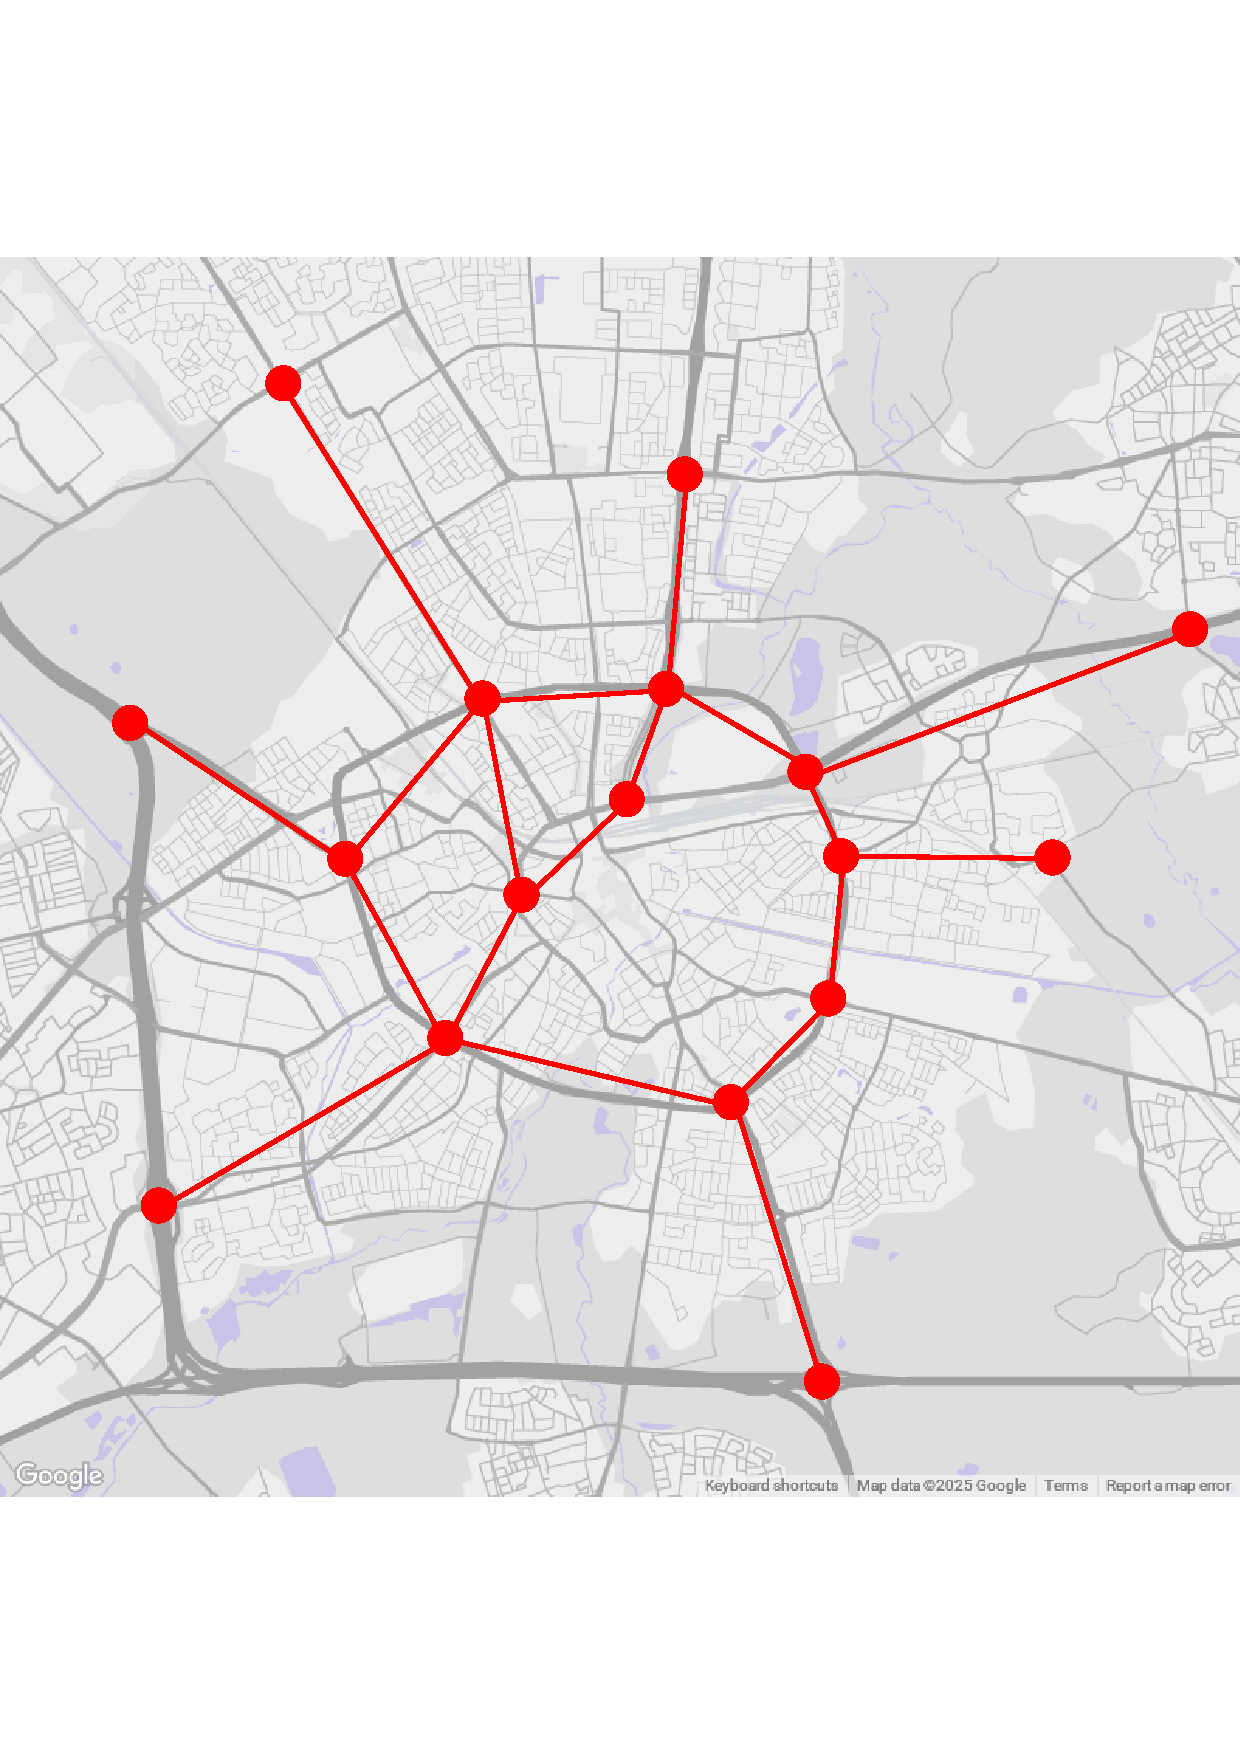
\includegraphics[trim={0 17px 0 0}, clip, width=.4\textwidth]{eindhoven-tsp.pdf}};

\draw[{Circle[fill=black,scale=0.6]}-] (Pe) ++(-0.2,-0.35) -- (eindhoven.north) ;

\node[inner sep=0pt] (montreal) at (3.0,-6)
    {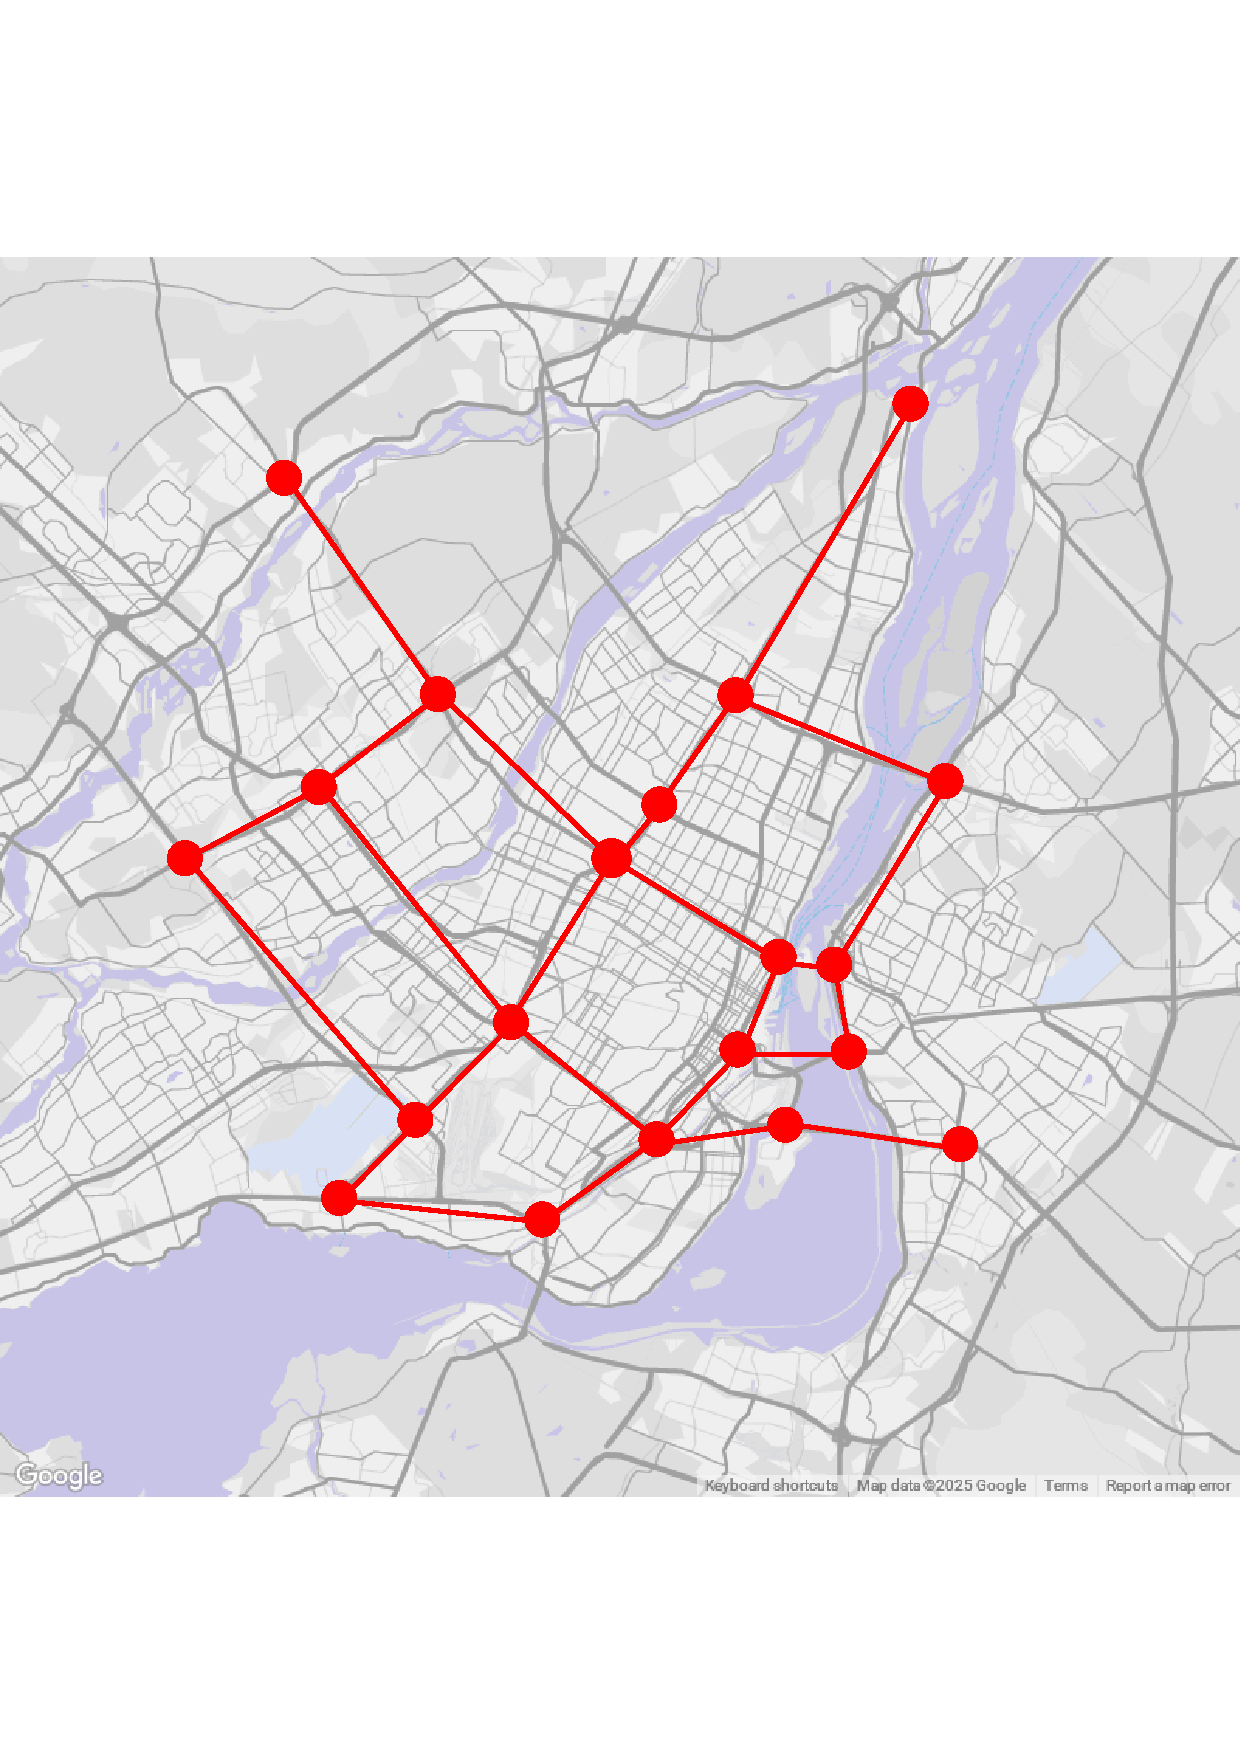
\includegraphics[trim={0 17px 0 0}, clip, width=.4\textwidth]{montreal-tsp.pdf}};

\draw[{Circle[fill=black,scale=0.6]}-] (Pm) ++(0.2,-0.4) -- (montreal) ;

\end{tikzpicture}
\end{document}
